\subsection{27. Алгоритм построения LR-таблицы. Вопрос на отл: доказательство корректности и полноты. Если верно определение, таблица строится и если не верно, не строится. Критерий LR-овости (отсутствие противоречий).}

\par \Def $A \rightarrow \alpha \cdot \beta, a_1 \ldots a_k$ - LR(k)-ситуация (неформально: если находимся в $A \rightarrow \alpha \cdot \beta$, то $a_1 \ldots a_k$ - первые буквы того, что можем вывести дальше, $a_i \in \Sigma \cup \{\$\}$)
\par \Note Далее будем рассматривать алгоритм LR(1), для $k \neq 1$ действуем аналогично.
\par \Def Пусть $I$ - множество ситуаций. Тогда $CLOSURE(I):=J, I \subset J$, такое что
$$\left.\begin{array}{c}
B \rightarrow \gamma \in P\\
A \rightarrow \alpha_1 \cdot B \alpha_2, a \in J\\
\end{array}
\right\} \Rightarrow \forall c \in First(\alpha_2 a): \: B \rightarrow \cdot \gamma, c \in J$$
\par \Def Пусть $I$ - множество ситуаций, $\lambda \in \Sigma \cup N$. Тогда $$GOTO(I, \lambda):=CLOSURE(\{\langle A \rightarrow \alpha_1 \lambda \cdot \alpha_2 \rangle \: | \: \langle A \rightarrow \alpha_1  \cdot\lambda \alpha_2 \rangle \in I\})$$
\begin{figure}[h]
\center{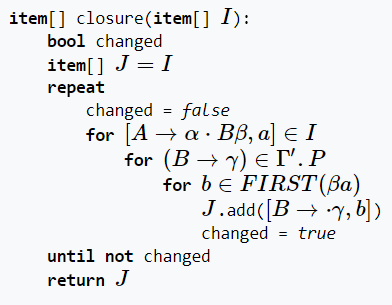
\includegraphics[scale=1]{images/LR(1)-closure.png}
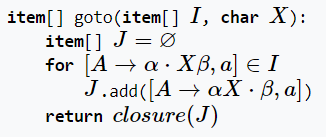
\includegraphics[scale=1]{images/LR(1)-goto.png}}
\end{figure}

\par Построим ДКА, вершинами которого будут множества ситуаций, а на ребрах будут написаны символы из $\Sigma \cup N$, по которым будем делать $GOTO$. Как строим: в начальное состояние добавляем $S' \rightarrow \cdot S, \$$. Затем берем $CLOSURE$ от состояния, делаем $GOTO$ по всем возможным буквам - получаем новые вершины автомата, в которые ведут ребра по этим буквам. Повторяем процесс для добавленных состояний и тд.
\begin{figure}[h]
\center{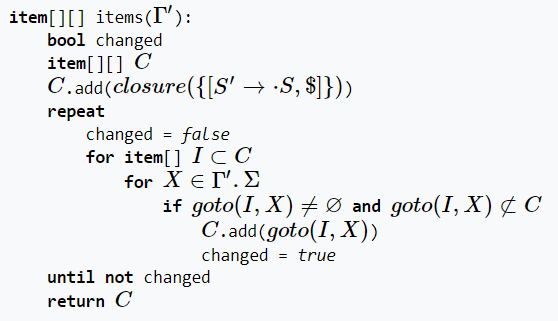
\includegraphics[scale=1]{images/LR(1)-automaton.png}}
\end{figure}
\\
\\
\\
\\
\\
\\
\\
\\


\par Теперь нам остается только построить таблицу $table$ по автомату (столбцы - символы из $N \cup \Sigma \cup \{\$\}$, строки - номера состояний в автомате):
\begin{enumerate}
    \item Если из состояния $i$ в состояние $j$ ведет ребро по букве $a$, то $table[i][a]=(shift, j)$.
    \item Если в состоянии $i$ есть ситуация $A \rightarrow \alpha \cdot, a$, то $table[i][a]=(reduce, j)$, где $j$ - номер правила $A \rightarrow \alpha$ в грамматике. Если нужно записать $(reduce, 0)$, то есть свертка по правилу $S' \rightarrow S$, то записываем $table[i][a]=accept$
    \item Если никакой из прошлых пунктов не записался, то $table[i][a]=error$
\end{enumerate}
\begin{figure}[h]
\center{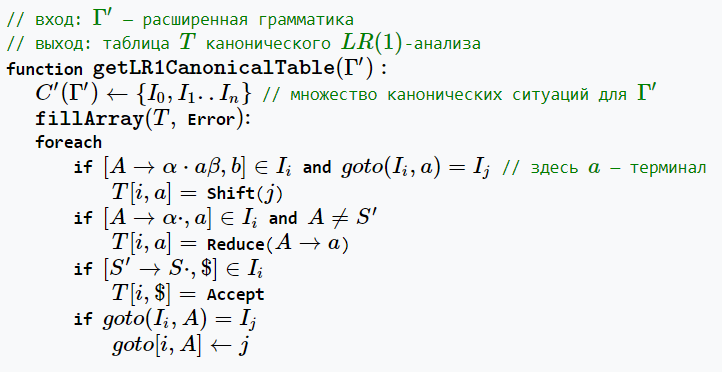
\includegraphics[scale=1]{images/LR(1)-table.png}}
\end{figure}